% !TEX root =  ../main.tex 

\section{Appendix}

\subsection{Personalized schedules for repeat biopsies}
In this section we present the derivations for Equation \ref{eq : expected_time_survprob} and Equation \ref{eq : var_time_survprob}. To this end, we first expand the formula for dynamic survival probability presented in Equation \ref{eq : dynamic_surv_prob}.
\begin{equation}
\label{eq : dyn_surv_prob_expanded}
\begin{split}
\pi_j(u \mid t, s) &= \mbox{Pr}\big\{T^*_j \geq u \mid  T^*_j >t, \mathcal{Y}_j(s\big\}, D_n)\\
&= \int \int \mbox{Pr}\big\{T^*_j \geq u \mid  T^*_j >t, \boldsymbol{b}_j,\boldsymbol{\theta}\big\} p\big(\boldsymbol{b}_j \mid T^*_j>t, \mathcal{Y}_j(s), \boldsymbol{\theta}\big)p\big(\boldsymbol{\theta} \mid \mathcal{D}_n\big) \diff \boldsymbol{b}_j \diff \boldsymbol{\theta}\\
&= \int \int \frac{\exp\big\{-H_j(u | \boldsymbol{b}_j, \boldsymbol{\theta})\big\}}{\exp\big\{-H_j(t | \boldsymbol{b}_j, \boldsymbol{\theta})\big\}} p\big(\boldsymbol{b}_j \mid T^*_j>t, \mathcal{Y}_j(s), \boldsymbol{\theta}\big)p\big(\boldsymbol{\theta} \mid \mathcal{D}_n\big) \diff \boldsymbol{b}_j \diff \boldsymbol{\theta}
\end{split}
\end{equation}
where $H_j(u | \boldsymbol{b}_j, \boldsymbol{\theta}) = \int_0^u h_i(s \mid \boldsymbol{b}_j, \boldsymbol{\theta}\big)\diff s$ is the cumulative hazard up to time point $u$.

\subsubsection{Derivation of Equation \ref{eq : expected_time_survprob}}
\label{subsubsec : deriv_eq_7}
\begin{equation*}
\begin{split}
E_g[T^*_j] &= \int_t^{\infty} T^*_j g(T^*_j)\diff T^*_j\\
\text{Using integration by parts, wherein} & \frac{\diff \big\{-\pi_j(T^*_j \mid t, s)\big\}}{\diff T^*_j} = g(T^*_j)\\
&= \Big[-T^*_j\pi_j(T^*_j \mid t, s)\Big]_t^\infty + \int_t^{\infty} \pi_j(T^*_j \mid t, s) \frac{\diff (T^*_j)}{\diff T^*_j} \diff T^*_j\\
&= t \pi_j(t \mid t, s) - \lim_{T^*_j\to \infty}T^*_j \pi_j(T^*_j \mid t, s) + \int_t^{\infty} \pi_j(T^*_j \mid t, s) \diff T^*_j\\
\end{split}
\end{equation*}
where $\pi_j(t \mid t, s) = \mbox{Pr}\big\{T^*_j \geq t \mid  T^*_j >t, \mathcal{Y}_j(s), D_n\big\} = 1$. As for $\lim_{T^*_j\to \infty}T^*_j \pi_j(T^*_j \mid t, s)$, the limit can be interchanged with the integral in Equation \ref{eq : dyn_surv_prob_expanded}, because as $T^*_j\to \infty$ the integrand in the equation converges uniformly on the domain of $(\boldsymbol{b}_j, \boldsymbol{\theta}\big)$. Thus,
\begin{equation*}
\begin{split}
\lim_{T^*_j\to \infty}T^*_j \pi_j(T^*_j \mid t, s) &=  \int \int \lim_{T^*_j\to \infty} \frac{T^*_j}{\exp\big\{H_j(T^*_j | \boldsymbol{b}_j, \boldsymbol{\theta})\big\}} \frac{p\big(\boldsymbol{b}_j \mid T^*_j>t, \mathcal{Y}_j(s), \boldsymbol{\theta}\big)p\big(\boldsymbol{\theta} \mid \mathcal{D}_n\big)}{\exp\big\{-H_j(t | \boldsymbol{b}_j, \boldsymbol{\theta})\big\}}  \diff \boldsymbol{b}_j \diff \boldsymbol{\theta}\\
\text{Using L'Hospital's rule}\\
\lim_{T^*_j\to \infty}T^*_j \pi_j(T^*_j \mid t, s) &=  \int \int \frac{1}{\lim_{T^*_j\to \infty} \exp\{H_j(T^*_j | \boldsymbol{b}_j, \boldsymbol{\theta}\big)\}H'_j(T^*_j | \boldsymbol{b}_j, \boldsymbol{\theta}\big)} \frac{p\big(\boldsymbol{b}_j \mid T^*_j>t, \mathcal{Y}_j(s), \boldsymbol{\theta}\big)p\big(\boldsymbol{\theta} \mid \mathcal{D}_n\big)}{\exp\{-H_j(t | \boldsymbol{b}_j, \boldsymbol{\theta}\big)\}} \diff \boldsymbol{b}_j \diff \boldsymbol{\theta}\\
&= \int \int 0 \frac{p\big(\boldsymbol{b}_j \mid T^*_j>t, \mathcal{Y}_j(s), \boldsymbol{\theta}\big)p\big(\boldsymbol{\theta} \mid \mathcal{D}_n\big)}{\exp\big\{-H_j(t | \boldsymbol{b}_j, \boldsymbol{\theta})\big\}}  \diff \boldsymbol{b}_j \diff \boldsymbol{\theta}\\
&= 0
\end{split}
\end{equation*}

In light of these results, we obtain:
\begin{equation*}
E_g[T^*_j] = t + \int_t^{\infty} \pi_j(T^*_j \mid t, s) \diff T^*_j\\
\end{equation*}

\subsubsection{Derivation of Equation \ref{eq : var_time_survprob}}
Since $\mbox{var}_g[T^*_j] = E_g[\{T^*_j\}^2] - E_g[T^*_j]^2$, we first show the derivation for $E_g[(T^*_j)^2]$.
\begin{equation*}
\begin{split}
E_g[(T^*_j)^2] &= \int_t^{\infty} (T^*_j)^2 g(T^*_j)\diff T^*_j\\
\text{Using integration by parts, wherein} & \frac{\diff \big\{-\pi_j(T^*_j \mid t, s)\big\}}{\diff T^*_j} = g(T^*_j)\\
E_g\big[\{T^*_j\}^2\big] &= \Big[-\{T^*_j\}^2\pi_j(T^*_j \mid t, s)\Big]_t^\infty + \int_t^{\infty} \pi_j(T^*_j \mid t, s) \frac{\diff (T^*_j)^2}{\diff T^*_j} \diff T^*_j\\
&= t^2 \pi_j(t \mid t, s) - \lim_{T^*_j\to \infty}(T^*_j)^2 \pi_j(T^*_j \mid t, s) + 2 \int_t^{\infty} T^*_j \pi_j(T^*_j \mid t, s) \diff T^*_j\\
&= t^2 + 2 \int_t^{\infty} T^*_j \pi_j(T^*_j \mid t, s) \diff T^*_j
\end{split}
\end{equation*}
Therefore,
\begin{equation*}
\begin{split}
\mbox{var}_g[T^*_j] &= t^2 + 2 \int_t^{\infty} T^*_j \pi_j(T^*_j \mid t, s) \diff T^*_j - \bigg[t^2 +  \Big\{\int_t^\infty \pi_j(T^*_j \mid t, s) \diff T^*_j \Big\}^2 + 2t\int_t^\infty \pi_j(T^*_j \mid t, s) \diff T^*_j \bigg]\\
&=2 \int_t^{\infty} (T^*_j - t) \pi_j(T^*_j \mid t, s) \diff T^*_j -  \Big\{\int_t^\infty \pi_j(T^*_j \mid t, s) \diff T^*_j \Big\}^2
\end{split}
\end{equation*}

\subsection{Simulation study}
This section presents the figures and tables for related to the simulation study results from Section \ref{sec: simulation_study}. More specifically:

\begin{itemize}
  \item Figure \ref{fig : meanNbVsOffset_G1}, Figure \ref{fig : meanNbVsOffset_G2} and Figure \ref{fig : meanNbVsOffset_G3} show plots of average number of biopsies against average offset for each of the 7 scheduling methods present in the simulation study.
  \item Figure \ref{fig : nbBoxPlot_G1} and Figure \ref{fig : offsetBoxPlot_G1} show boxplots of number of biopsies and offset for each of the 6 scheduling methods for the patients in subgroup $G_1$. Similar plots for subgroup $G_2$ and $G_3$ are shown in Figure \ref{fig : nbAndOffsetBoxPlot_G2} and Figure \ref{fig : nbAndOffsetBoxPlot_G3} respectively.
  \item Figure \ref{fig : nbMeanBoxPlot_all} and Figure \ref{fig : offsetMeanBoxPlot_all} show the variation in estimated mean number of biopsies and estimated mean offset computed during the 254 simulations, for patients from all subgroups. The same plots for each of the subgroups are shown in Figure \ref{fig : nbAndOffsetMeanBoxPlot_G1}, Figure \ref{fig : nbAndOffsetMeanBoxPlot_G2} and Figure \ref{fig : nbAndOffsetMeanBoxPlot_G3}.
\end{itemize} 

\begin{figure}[!htb]
    \centering
    \captionsetup{justification=centering}
     \begin{subfigure}[b]{0.45\textwidth}
        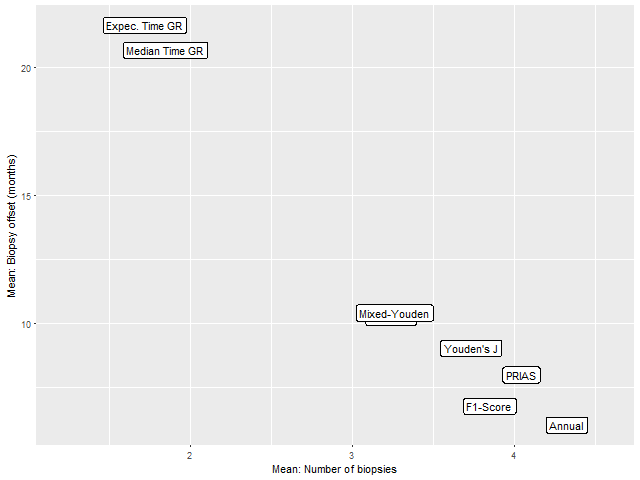
\includegraphics[width=\textwidth]{images/sim_study/meanNbVsOffset_scale_4.png}
		\caption{Plot for subgroup $G_1$}
		\label{fig : meanNbVsOffset_G1}
    \end{subfigure}
    \begin{subfigure}[b]{0.45\textwidth}
		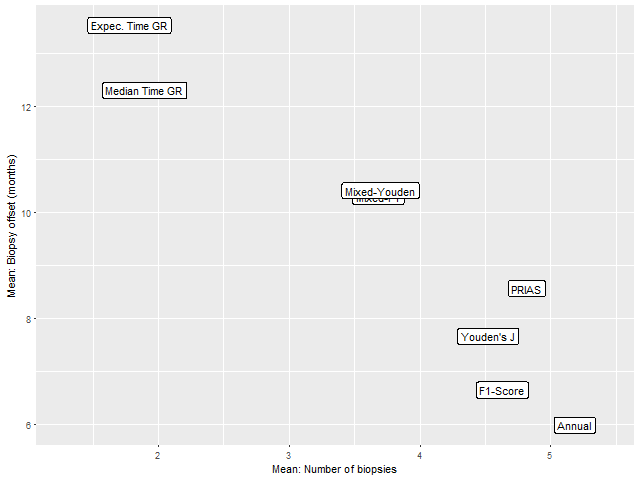
\includegraphics[width=\textwidth]{images/sim_study/meanNbVsOffset_scale_5.png}
		\caption{Plot for subgroup $G_2$}
		\label{fig : meanNbVsOffset_G2}
    \end{subfigure}  
    \begin{subfigure}[b]{0.45\textwidth}
		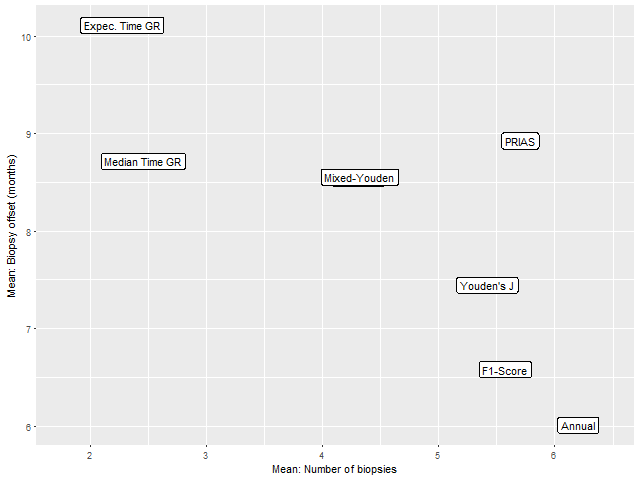
\includegraphics[width=\textwidth]{images/sim_study/meanNbVsOffset_scale_6.png}
		\caption{Plot for subgroup $G_3$}
		\label{fig : meanNbVsOffset_G3}
    \end{subfigure}      
    \caption{Estimated mean number of biopsies and mean offset (months) for the 7 scheduling methods for the 3 sub-groups. Method names are abbreviated for ease of graphing.}
\end{figure}

\begin{figure}[!htb]
    \centering
    \captionsetup{justification=centering}
     \begin{subfigure}[b]{0.45\textwidth}
        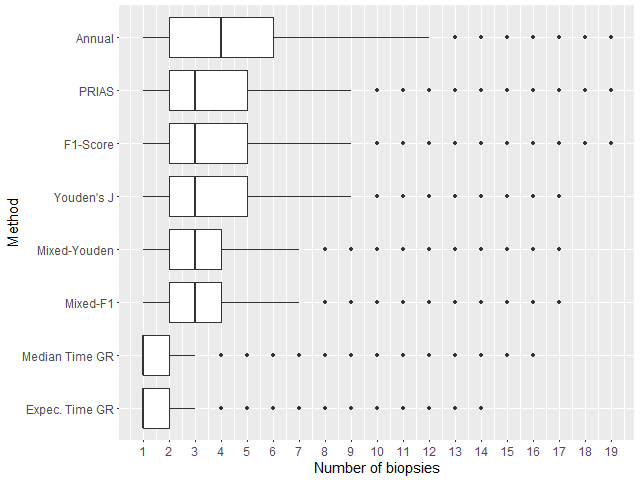
\includegraphics[width=\textwidth]{images/sim_study/nbBoxPlot_scale_4.png}
        \caption{Boxplot for number of biopsies.}
        \label{fig : nbBoxPlot_G1}
    \end{subfigure}
    \begin{subfigure}[b]{0.45\textwidth}
        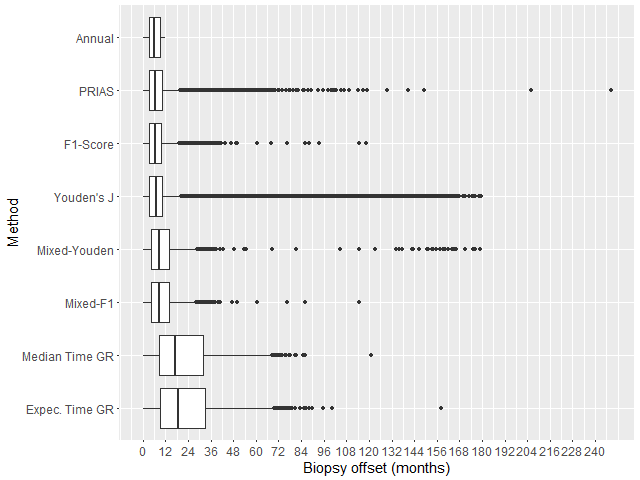
\includegraphics[width=\textwidth]{images/sim_study/offsetBoxPlot_scale_4.png}
        \caption{Boxplot for offset (months)}
        \label{fig : offsetBoxPlot_G1}
    \end{subfigure}      
    \caption{Boxplot for number of biopsies and offset (months), for all patients in subgroup $G_1$ across all simulations. Method names are abbreviated for ease of graphing.}
    \label{fig : nbAndOffsetBoxPlot_G1}
\end{figure}

\begin{figure}[!htb]
    \centering
    \captionsetup{justification=centering}
     \begin{subfigure}[b]{0.45\textwidth}
        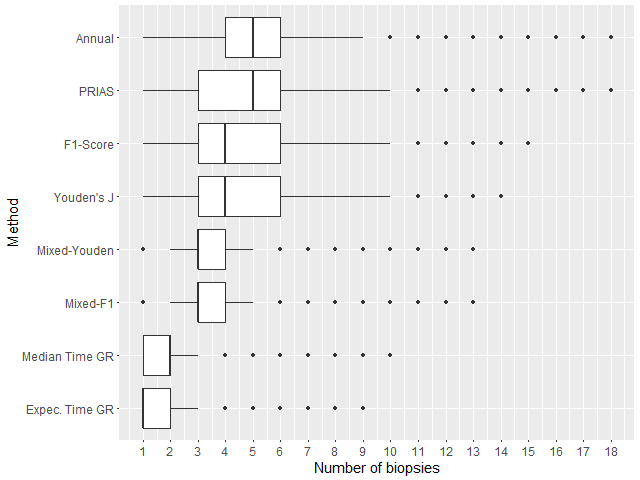
\includegraphics[width=\textwidth]{images/sim_study/nbBoxPlot_scale_5.png}
        \caption{Boxplot for number of biopsies.}
        \label{fig : nbBoxPlot_G2}
    \end{subfigure}
    \begin{subfigure}[b]{0.45\textwidth}
        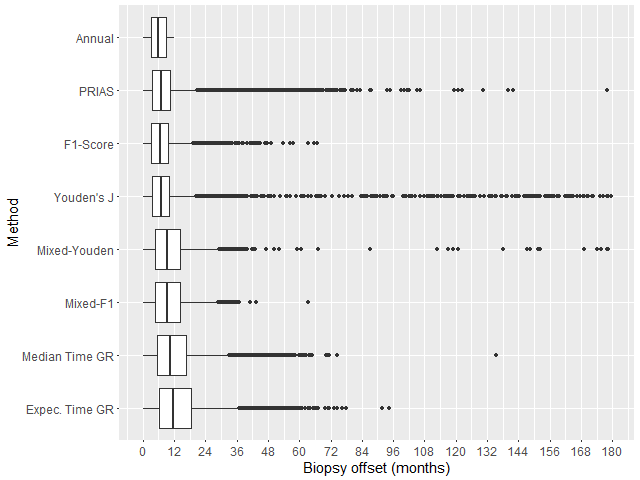
\includegraphics[width=\textwidth]{images/sim_study/offsetBoxPlot_scale_5.png}
        \caption{Boxplot for offset (months)}
        \label{fig : offsetBoxPlot_G2}
    \end{subfigure}      
    \caption{Boxplot for number of biopsies and offset (months), for all patients in subgroup $G_2$ across all simulations. Method names are abbreviated for ease of graphing.}
     \label{fig : nbAndOffsetBoxPlot_G2}
\end{figure}

\begin{figure}[!htb]
    \centering
    \captionsetup{justification=centering}
     \begin{subfigure}[b]{0.45\textwidth}
        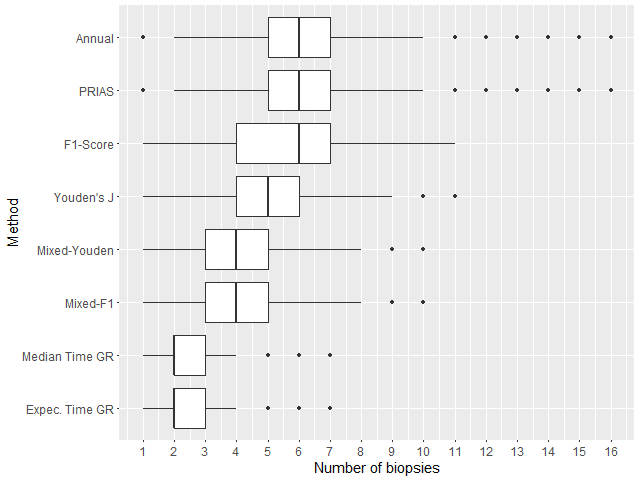
\includegraphics[width=\textwidth]{images/sim_study/nbBoxPlot_scale_6.png}
        \caption{Boxplot for number of biopsies.}
        \label{fig : nbBoxPlot_G3}
    \end{subfigure}
    \begin{subfigure}[b]{0.45\textwidth}
        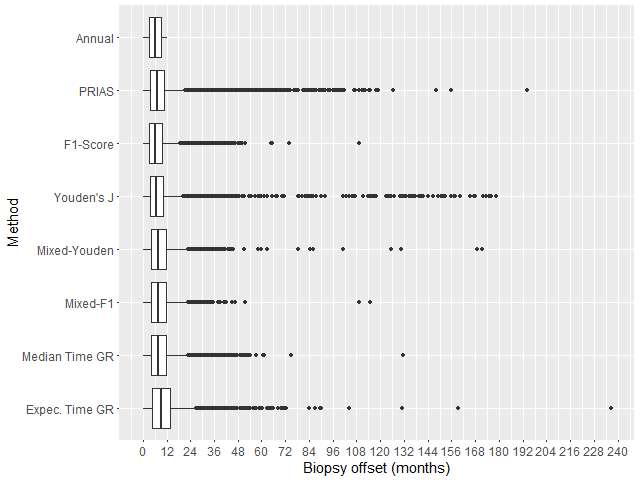
\includegraphics[width=\textwidth]{images/sim_study/offsetBoxPlot_scale_6.png}
        \caption{Boxplot for offset (months)}
        \label{fig : offsetBoxPlot_G3}
    \end{subfigure}      
    \caption{Boxplot for number of biopsies and offset (months), for all patients in subgroup $G_3$ across all simulations. Method names are abbreviated for ease of graphing.}
     \label{fig : nbAndOffsetBoxPlot_G3}
\end{figure}

\begin{figure}[!htb]
    \centering
    \captionsetup{justification=centering}
     \begin{subfigure}[b]{0.45\textwidth}
        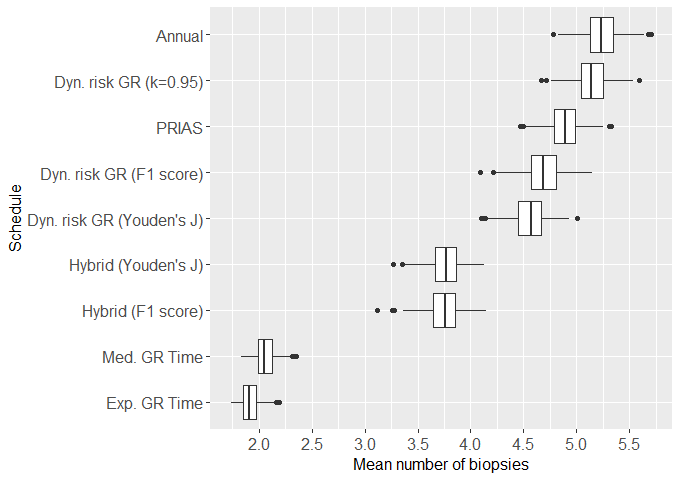
\includegraphics[width=\textwidth]{images/sim_study/nbMeanBoxPlot_all.png}
        \caption{Boxplot for mean number of biopsies.}
        \label{fig : nbMeanBoxPlot_all}
    \end{subfigure}
    \begin{subfigure}[b]{0.45\textwidth}
        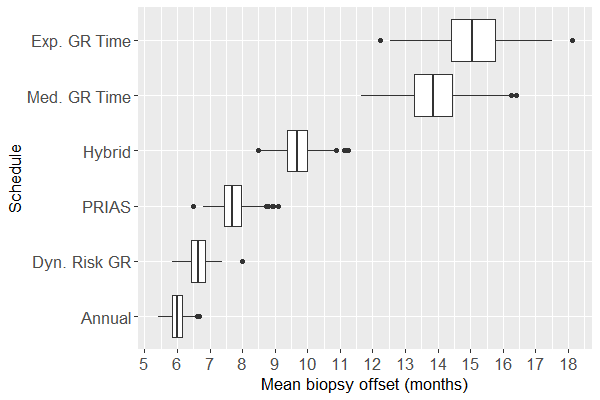
\includegraphics[width=\textwidth]{images/sim_study/offsetMeanBoxPlot_all.png}
        \caption{Boxplot for mean offset (months)}
        \label{fig : offsetMeanBoxPlot_all}
    \end{subfigure}      
    \caption{Boxplot showing variation in mean number of biopsies and mean offset (months) for all of the patients across the 254 simulations.}
\end{figure}

\begin{figure}[!htb]
    \centering
    \captionsetup{justification=centering}
     \begin{subfigure}[b]{0.45\textwidth}
        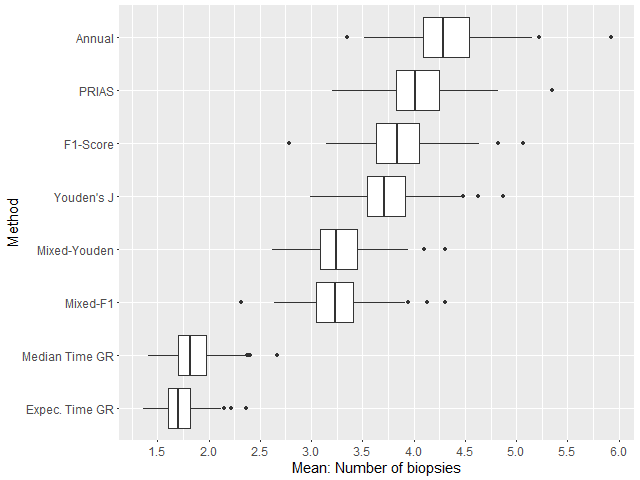
\includegraphics[width=\textwidth]{images/sim_study/nbMeanBoxPlot_scale_4.png}
        \caption{Boxplot for mean number of biopsies.}
        \label{fig : nbMeanBoxPlot_G1}
    \end{subfigure}
    \begin{subfigure}[b]{0.45\textwidth}
        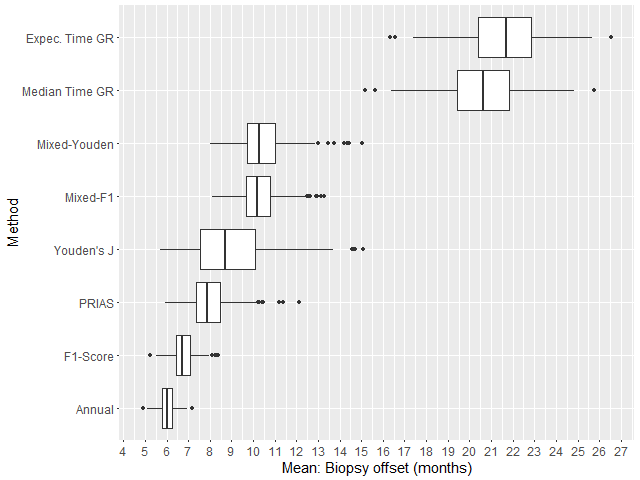
\includegraphics[width=\textwidth]{images/sim_study/offsetMeanBoxPlot_scale_4.png}
        \caption{Boxplot for mean offset (months)}
        \label{fig : offsetMeanBoxPlot_G1}
    \end{subfigure}      
    \caption{Boxplot showing variation in mean number of biopsies and mean offset (months) for patients in subgroup $G_1$ across the 254 simulations.}
    \label{fig : nbAndOffsetMeanBoxPlot_G1}
\end{figure}

\begin{figure}[!htb]
    \centering
    \captionsetup{justification=centering}
     \begin{subfigure}[b]{0.45\textwidth}
        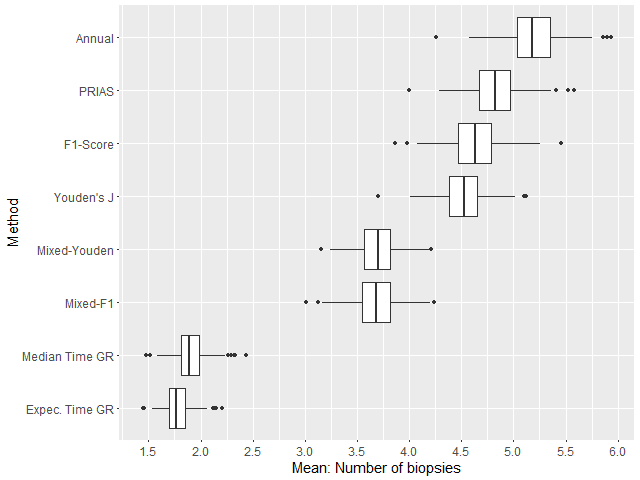
\includegraphics[width=\textwidth]{images/sim_study/nbMeanBoxPlot_scale_5.png}
        \caption{Boxplot for mean number of biopsies.}
        \label{fig : nbMeanBoxPlot_G2}
    \end{subfigure}
    \begin{subfigure}[b]{0.45\textwidth}
        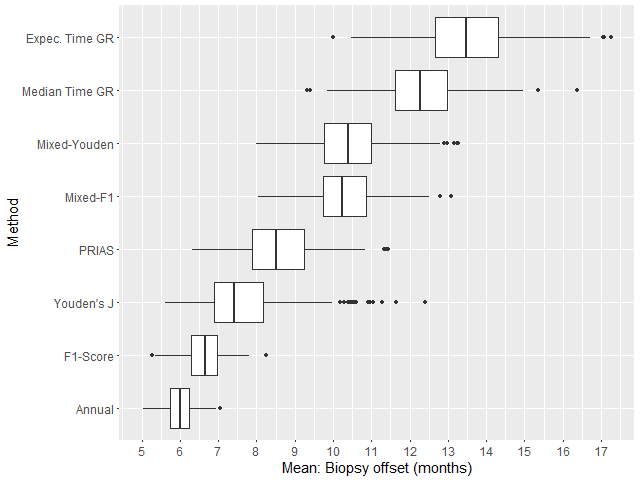
\includegraphics[width=\textwidth]{images/sim_study/offsetMeanBoxPlot_scale_5.png}
        \caption{Boxplot for mean offset (months)}
        \label{fig : offsetMeanBoxPlot_G2}
    \end{subfigure}      
    \caption{Boxplot showing variation in mean number of biopsies and mean offset (months) for patients in subgroup $G_2$ across the 254 simulations.}
    \label{fig : nbAndOffsetMeanBoxPlot_G2}
\end{figure}

\begin{figure}[!htb]
    \centering
    \captionsetup{justification=centering}
     \begin{subfigure}[b]{0.45\textwidth}
        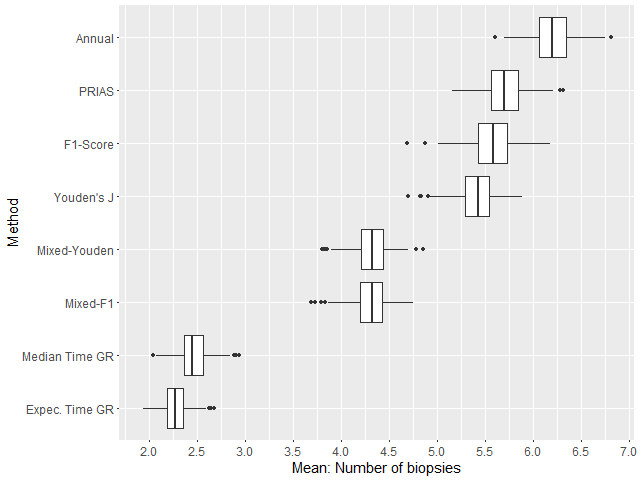
\includegraphics[width=\textwidth]{images/sim_study/nbMeanBoxPlot_scale_6.png}
        \caption{Boxplot for mean number of biopsies.}
        \label{fig : nbMeanBoxPlot_G3}
    \end{subfigure}
    \begin{subfigure}[b]{0.45\textwidth}
        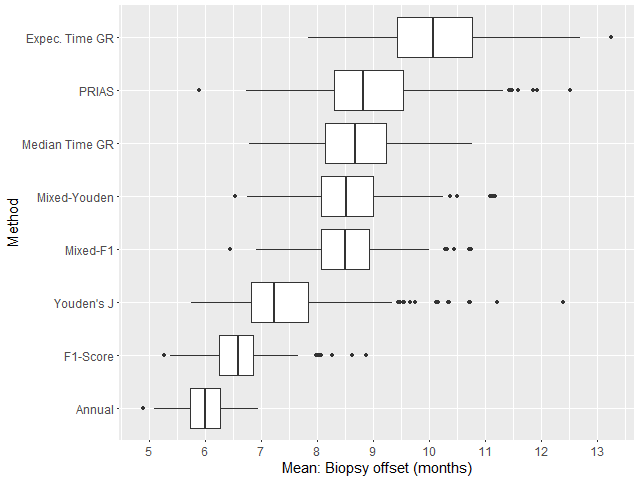
\includegraphics[width=\textwidth]{images/sim_study/offsetMeanBoxPlot_scale_6.png}
        \caption{Boxplot for mean offset (months)}
        \label{fig : offsetMeanBoxPlot_G3}
    \end{subfigure}      
    \caption{Boxplot showing variation in mean number of biopsies and mean offset (months) for patients in subgroup $G_3$ across the 254 simulations.}
    \label{fig : nbAndOffsetMeanBoxPlot_G3}
\end{figure}